\newpage
\section{Introduzione} \label{Introduzione}
	
	\subsection{Scopo del documento}
	Questo documento ha l'intento di specificare la \gloss{pianificazione} e l'approccio che \gruppo adotterà per portare a termine il progetto Butterfly.
	All'interno vengono illustrate le strategie, le suddivisioni dei compiti, l'utilizzo delle risorse, la gestione dei rischi e le attività secondo le quali il team di sviluppo ha intenzione di lavorare.
	
	\subsection{Scopo del prodotto}	
	Il prodotto che \gruppo\ si incarica di realizzare è Butterfly: un tool di supporto alle figure di sviluppo in aziende che producono software (non solamente quella del committente).
	Questo applicativo permette di incanalare le notifiche dei vari strumenti utilizzati nel percorso di \gloss{CI} e \gloss{CD} (come Redmine, GitLab, ecc.) di un software e, tramite un \gloss{broker} (\gloss{Apache Kafka} in questo caso), spedirli alla persona interessata tramite il canale di comunicazione
	preferito scelto da quest'ultimo (email, Telegram, Slack, ecc.).
	
	\subsection{Glossario}
		\subsubsection{Riferimenti Normativi}
			\begin{itemize}
				\item \textbf{Capitolato d'appalto C1}: presentazione del capitolato C1;\\
				\url{https://www.math.unipd.it/~tullio/IS-1/2018/Progetto/C1.pdf}
				\item \textbf{Vincoli di organigramma e specifiche economiche}\\
				\url{https://www.math.unipd.it/~tullio/IS-1/2018/Progetto/RO.html}
				\item \textbf{Norme di progetto interne di \gruppo}: \NdPv;
				\item \textbf{The twelve factor app}: norme per lo sviluppo di un prodotto software consigliate dall'azienda.\\
				\url{https://12factor.net/}
			\end{itemize}
		
		\subsubsection{Riferimenti Informativi}
			\begin{itemize}
				\item \textbf{Software Engineering - Ian Sommerville - 10 th Edition (2016)}
				\item \textbf{Slide dell’insegnamento Ingegneria del Software}\\
				\url{http://www.math.unipd.it/~tullio/IS-1/2018/}
				\item \textbf{I sistemi per la gestione dei rischi}: presentazione rilasciata dalla Bocconi per la gestione dei rischi.\\
				\url{https://www2.deloitte.com/content/dam/Deloitte/it/Documents/risk/Board\%20Academy\%20Corso\%20C6\%2020\%20dic\%202012\%20SDA\%20Bocconi.pdf}
			\end{itemize}
		
	\subsection{Scadenze}
	\gruppo\ ha deciso di rispettare le scadenze indicate dal professor Vardanega e riportate di seguito:
	\begin{itemize}
		\item \textbf{Revisione dei Requisiti}: 21-01-2019;
		\item \textbf{Revisione di Progetto}: 15-03-2019;
		\item \textbf{Revisione di Qualifica}: 19-04-2019;
		\item \textbf{Revisione di Accettazione}: 17-05-2019.
	\end{itemize}
	
	\subsection{Ciclo di vita} % Usare modello di sviluppo come termine al posto di Ciclo di vita in questo contesto. Vedere #26
	Data la natura del progetto, composto da più parti modulari e quindi con un valore basso di accoppiamento, il team di sviluppo ha stabilito di adottare un ciclo di vita con un modello ibrido tra quello a componenti e quello incrementale.
	Questi modelli si adattano particolarmente a questo tipo di progetto in quanto:
	\begin{itemize}
		\item il modello incrementale prevede ripetizioni identificate come cicli di incremento che verranno ripetute fino a quando il prodotto non arriverà a soddisfare i requisiti richiesti dal cliente;
		\item il modello a componenti è basato sul riuso di unità software che possono avere diverse dimensione:
		\begin{itemize}
			\item \textbf{System reuse}: un intero sistema, composto da più applicazioni, può essere riusato come parte di un sistema di tanti sistemi;
			\item \textbf{Application reuse}: un'applicazione può essere riusata incorporandola in altri sistemi senza apportare cambiamenti, oppure configurandola;
			\item \textbf{Component reuse}: i componenti di un'applicazione, che possono essere dai da sotto-sistemi ai singoli oggetti, risiedono in un cloud o in server privati e possono essere accessibili tramite Application Programming Interface (API); 
			\item \textbf{Object and function reuse}: componenti software che implementano una singola funzione o una classe oggetto si possono riusare collegandole con lo sviluppo di nuovo codice. Molte di queste sono liberamente disponibili. 
		\end{itemize}
		Oppure, nel caso in cui le componenti siano così specifiche da essere molto costoso adattarle ad una nuova situazione, è possibile fare "concept reuse", ovvero riusare le idee che stanno alla base del componente (e.g. riusare un \gloss{way of working} o un algoritmo). \par
		In particolare i benefici che si possono trarre dal riuso sono:
		\begin{itemize}
			\item \textbf{Costo complessivo di sviluppo più basso}: perché il numero di componenti software che devono essere progettati, implementati e validati è minore;
			\item \textbf{Sviluppo accelerato}
			\item \textbf{Aumento dell'affidabilità}: un software che è stato provato e testato in altri sistemi risulta più affidabile di un software appena implementato. I suoi difetti di progettazione e implementazione dovrebbero già esser stati individuati e risolti;
			%\item  Ridotto rischio di processo, vero specialmente per grandi componenti software riusate come sottosistemi. È un fattore importante per il Project Manager perché riduce il margine di errore nella stima dei costi di un progetto.
			\item \textbf{Conformità con gli standard}: alcuni standard
			%, come gli interface standard, 
			possono essere implementati come set di componenti riusabili.
		\end{itemize}
		%e prevede che venga riutilizzata una base per lo sviluppo dei vari pezzi che formano il progetto, fra loro indipendenti;
	\end{itemize}
	Inizialmente quindi si potranno spendere le risorse nella realizzazione di una base di partenza per i componenti, che verrà successivamente sviluppata per ciascun requisito richiesto rappresentando il core del prodotto finale.
	A tale \gloss{milestone} si potranno integrare le funzionalità secondarie richieste dal cliente insieme ai possibili requisiti impliciti desiderabili presenti nel capitolato. In base alla pianificazione svolta, le risorse disponibili saranno ridistribuite in modo da garantire lo sviluppo completo del prodotto.
	L'immagine che segue rappresenta il modello incrementale e come il progetto viene composto da componenti sviluppati ciascuno secondo cicli con fasi ben definite.
	\begin{figure}[H]
		\centering
		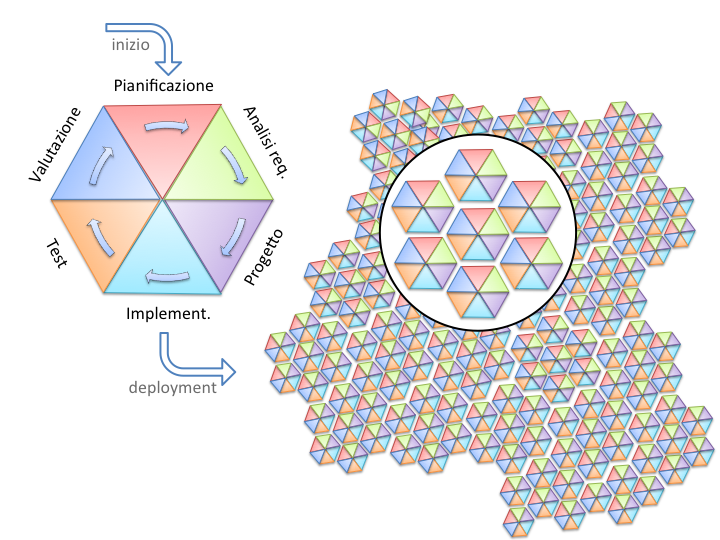
\includegraphics[scale=0.5]{img/modello_incrementale.png}
		\caption{Rappresentazione del modello incrementale \protect\footnotemark}
	\end{figure}

	\footnotetext{Fonte: \url{https://it.wikipedia.org/wiki/Modello_incrementale}}
	